\chapter{Streaming assembly using Nanopore reads}\label{ch:npscarf}
\thispagestyle{empty}
\vspace*{\fill}
\epigraph{\emph{The speed of decision making is the essence of good governance.}}
{--Piyush Goyal}

\clearpage
%%%%%%%%%%%%%%%%%%%%%%%%%%%%%%%%%%%%%%%%%%%%%%%%
This chapter describes a unique streaming assembly strategy on MinION data that has been implemented in a tool named \npscarf{}. Its methodology allows completing the assembly in real-time together with the nanopore sequencing nature. Several experiments on different data sets are conducted for better illustrations of \npscarf{} performance and functionality. 
Comparisons with other methods indicate better quality from the results while at the same time, consume less resources and running time.

These research findings have been published in a journal manuscript under the digital object identifier (DOI):$\mathtt{10.1038/ncomms14515}$. The manuscript will be reproduced with minor changes and reformatting for the whole content of this chapter.
The Supplementary materials for this paper is shown in \App{app:npscarf}.

As the co-first author, I am a primary contributor to the project in term of conception and design, software development, data analysis as well as drafting the first version of the manuscript. 
Specifically, I have predominantly designed the streaming pipeline and implemented the algorithm as the main developer of \npscarf{}. 
I have also contributed significantly to the analysis and interpretation of the research data. 
Finally, I am the author of the first draft versions of the manuscript on which the publication is based.

\clearpage
%%%%%%%%%%%%%%%%%%%%%%%%%%%%%%%%%%%%%%%%%%%%%%%%
%%%%%%%%%%%%%%%%%%%% Paper %%%%%%%%%%%%%%%%%%%%%
%\pagebreak
\thispagestyle{empty}
\vskip36pt
{\raggedright\sffamily\bfseries\fontsize{20}{25}\selectfont {Scaffolding and completing genome assemblies in real-time with nanopore sequencing}\par}
\vskip20pt
{\raggedright\sffamily\fontsize{12}{12}\usefont{OT1}{phv}{m}{n} {
\textbf{Minh Duc Cao}\textsuperscript{1,$\ast$,+},
\textbf{Son Hoang Nguyen}\textsuperscript{1,+},
\textbf{Devika Ganesamoorthy}\textsuperscript{1},
\textbf{Alysha G. Elliott}\textsuperscript{1},
\textbf{Matthew A.  Cooper}\textsuperscript{1} and
\textbf{Lachlan J.M. Coin}\textsuperscript{1,$\ast$}
}\par}
\vskip10pt
{\raggedright\sffamily\fontsize{10}{12}\usefont{OT1}{phv}{m}{n} {
\textsuperscript{1}Institute for Molecular Bioscience, University of Queensland, 
St Lucia, Brisbane, QLD 4072 Australia \par
\textsuperscript{$\ast$}Correspondence: \href{m.cao1@uq.edu.au}{m.cao1@uq.edu.au} and \href{l.coin@imb.uq.edu.au}{l.coin@imb.uq.edu.au} \par 
\textsuperscript{+}These authors contributed equally to this work
}\par}
\vskip10pt
{\raggedright\sffamily\fontsize{12}{16}\selectfont  {Received 11 Jul 2016. Accepted 6 Jan 2017. Published 20 Feb 2017}\par}
\vskip10pt
{\raggedright\sffamily\fontsize{12}{16}\selectfont  
PMID: 28218240 \hskip15pt DOI:~\href{https://doi.org/10.1038/ncomms14515}{10.1038/ncomms14515}\par}
\vskip10pt
\paragraph{Abstract}\mbox{}\\
Third generation sequencing technologies provide the opportunity to improve
genome assemblies by generating long reads spanning most repeat sequences. 
However, current analysis methods require substantial amounts of sequence data and
computational resources to overcome the high error rates. Furthermore, they can
only perform analysis after sequencing has completed, resulting in
either over-sequencing, or in a low quality assembly due to under-sequencing. Here we
present \npscarf{}, which can scaffold and complete short read assemblies while the
long read sequencing run is in progress. It reports assembly metrics in real-time so
the sequencing run can be terminated once an assembly of sufficient quality is
obtained. In assembling four bacterial and one eukaryotic genomes, we show that
\npscarf{} can construct more complete and accurate assemblies while requiring less
sequencing data and computational resources than existing methods. Our approach
offers a time- and resource-effective strategy for completing short read
assemblies.
\clearpage
\pagebreak

\section{Introduction}

High-throughput sequencing technology has transformed genomics research over the
last decade with the ability to sequence the whole genome of virtually any
organism on the planet. Most sequencing projects to date employ short read
technology and hence cannot unambiguously resolve the repetitive sequences that
are present abundantly in most genomes. As a result, assemblies are fragmented
into large numbers of contigs and the positions of repeat sequences in the
genome cannot be determined. These repeat sequences often play important
biological roles; for example, they mediate the lateral transfer of genes
between bacterial species via pathogenicity islands and plasmids. Analysing
these regions is thus essential to determine key characteristics such as
antimicrobial resistance (AMR) or to identify highly pathogenic variants of many
bacterial species~\cite{AshtonND2015}.

Long read sequencing technologies, for example Pacific Biosciences' (PacBio) and
Oxford Nanopore MinION sequencing, allow users to generate reads spanning most
repetitive sequences, which can be used to close gaps in fragmented assemblies.
A key innovation of the MinION nanopore sequencing device is that it
measures the changes in electrical current as a single-stranded molecule of DNA
passes through the nanopore and uses the signal to determine the nucleotide
sequence of the DNA strand~\cite{KasianowiczBB1996, BrantonDM2008, StoddartHM2009}. 
As such, the raw data of a read can be retrieved and analysed
as soon as it is generated, while sequencing of other reads is
still in progress.
This offers the opportunity to obtain analysis results as
soon as sufficient data are generated, upon which sequencing can be terminated
or used for other experiments.

Several algorithms have been developed to utilise long reads for genome
assembly. \emph{de novo} assemblers such as the hierarchical genome assembly
process (HGAP)~\cite{ChinAM2013} and nanocorrect/nanopolish~\cite{LomanQS2015}
can assemble a complete bacterial genome using only long read sequencing data.
However, because of the high error rates in these sequencing technologies, this
\emph{de novo} approach requires substantial amounts of sequencing data and
extensive computational resources, mainly for polishing the genome assembly. 
Hybrid assemblers, which combine error-prone long reads with highly accurate
and cheaper short read sequence data, provide a more economical and efficient
alternative for building complete genomes. They can be classified into three
categories. \emph{de novo} methods such as Canu~\cite{BerlinKC2015} and
miniasm/racon pipeline~\cite{Vaser2017racon} employ fast approximate approaches to assemble a skeleton of the genome using long reads. The skeleton, often as erroneous as the raw reads, is then polished with high quality short reads. On the other hand, tools in the \emph{error-correction} category (\EG, PBcR~\cite{KorenSW2012}, Nanocorr~\cite{GoodwinGE2015} and NaS~\cite{MadouiEC2015}) correct long reads with high quality short reads before assembling the genome with the corrected long reads. Finally, the \emph{scaffolding} methods (SPAdes-hybrid~\cite{BankevichNA2012, AshtonND2015},
SSPACE-LongRead~\cite{BoetzerP2014, KarlssonLS2015} and LINKS~\cite{WarrenYV2015}) use long reads to scaffold and fill in gaps in the
assemblies from short read sequencing.

While these tools are reported to assemble high quality bacterial
genomes~\cite{Castro-WallaceCJ2016, IstaceFD2016}, they have not made use of
the real-time sequencing potential of the MinION; assembly of a genome can only
be performed after the sequencing is complete. This can lead to over-sequencing,
which incurs extra cost and time; or under-sequencing resulting in a low-quality
assembly. Here, we present \npscarf{}, the first hybrid assembler that can
scaffold and complete fragmented short read assemblies with sequence data
streaming from the MinION while sequencing is still in progress. 
In effect, \npscarf{} can fully utilise a sequence read within
minutes of it being generated. Furthermore, it continuously reports
assembly quality during the experiment so that users can terminate the sequencing 
when an assembly of sufficient quality and completeness is obtained.
We show that our method can generate more accurate and more
complete genomes than existing tools, while requiring less nanopore sequencing
data and computational resources. As such, \npscarf{} can be used to efficiently
control MinION sequencing in completing existing short read assemblies and in
hybrid assembly projects. More importantly, \npscarf{} can facilitate the
real-time analysis of positioning genomic sequences for time critical
applications such as in AMR investigation.
We show that the \npscarf{} can rapidly and accurately reconstruct genomic islands
carrying AMR genes that are fragmented in short read assemblies. It can also
identify AMR genes encoded in plasmids. These are among the main analyses to
understand the acquisition of AMR in pathogenic bacteria.


\section{Results}

\subsection{Algorithm overview}

\begin{figure}[ht]
\centering
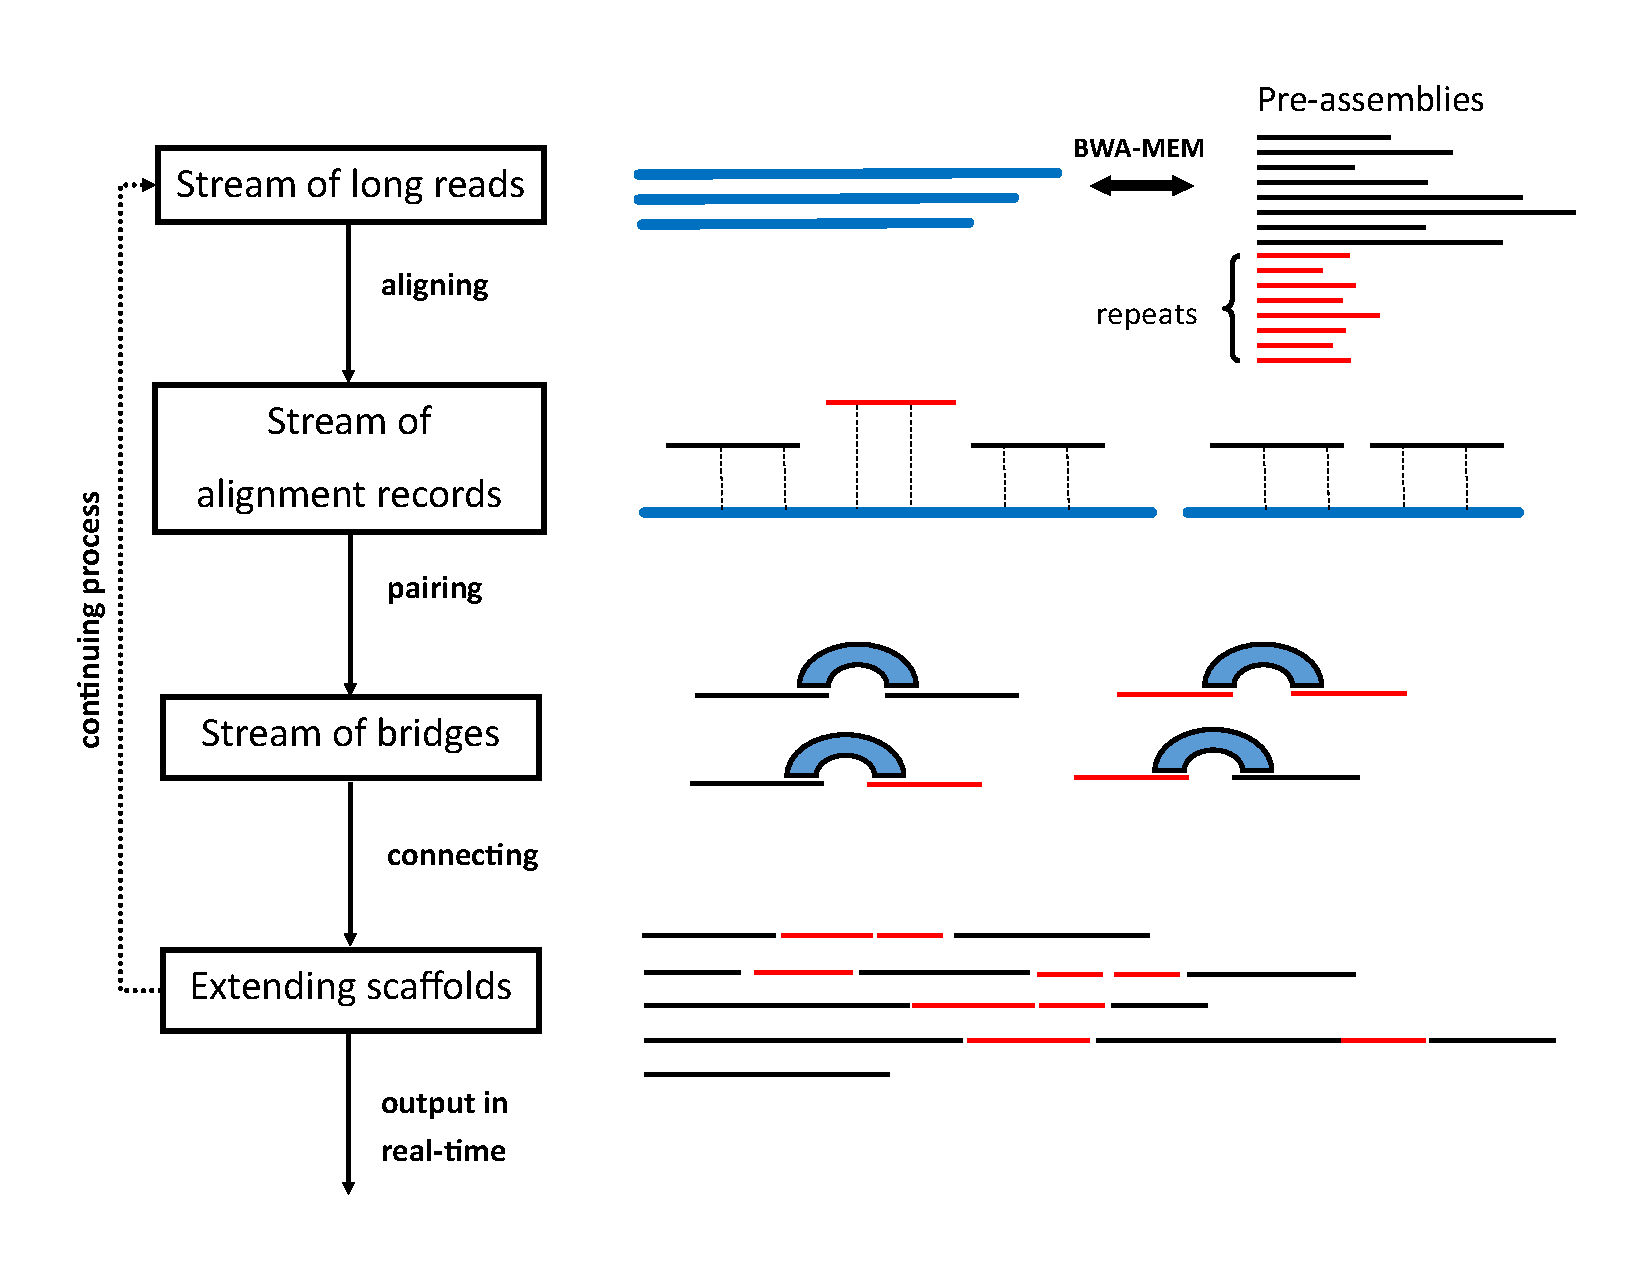
\includegraphics[width=\linewidth]{npscarf/figures/figure1.pdf}
\caption[Workflow of the real-time algorithm]{
Workflow of the real-time algorithm. Stream of long reads are aligned to the
existing contigs to create alignment records. Bridges connecting contigs are 
formed, and are used for extending scaffolds. These steps are performed in a
streaming fashion.}
\label{f:workflow}
\end{figure}

The genomes of most organisms contain an abundance of repeat sequences that are 
longer than the read length limit (300 bps) of Illumina sequencing 
platforms~\cite{TreangenS2012}. In assembling a genome using this technology, 
these repeat sequences cannot be distinguished and hence are often collapsed
into contigs, leaving gaps in the genome assembly. To complete the assembly, 
\npscarf{} first determines the multiplicity of each contig, thereby identifying
contigs representing non-repetitive sequences (called unique contigs).
It then scaffolds  and fills in gaps in the assembly in a streaming fashion
(Figure~\ref{f:workflow}). Upon receiving a long read from the MinION, \npscarf{}
immediately aligns it to the unique contigs. Reads aligned to two unique contigs
form a bridge connecting the two contigs. Gradually, the unique contigs are
joined to form the scaffold of the genome, while the repetitive contigs are
used to fill in the gaps in the scaffold. The details of the algorithms are
presented in Methods.

\subsection{Completing bacterial assemblies} 
\begin{figure*}[ht]
\centering
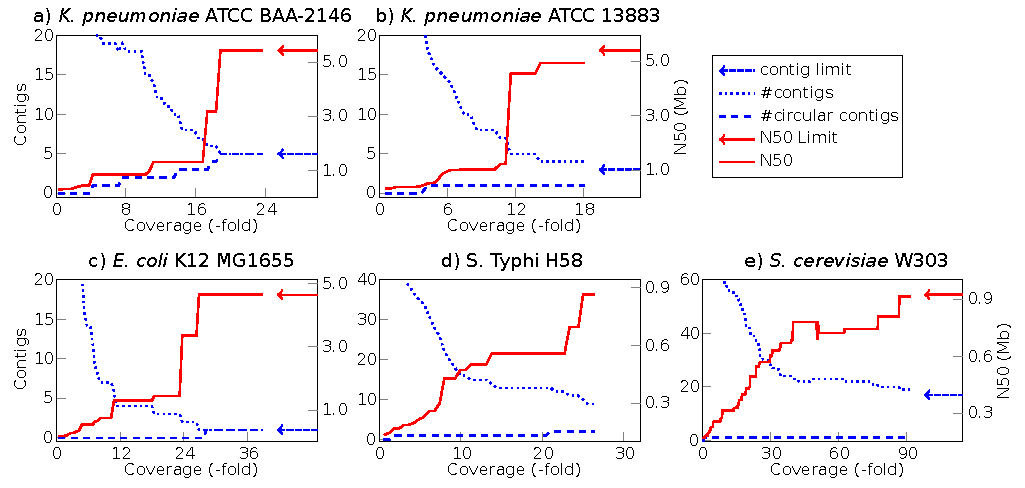
\includegraphics[width=\linewidth]{npscarf/figures/figure2.pdf}
\caption[Assembly statistics during real-time scaffolding]
{Assembly statistics during real-time scaffolding. 
The plots show N50 statistics, number of contigs, and number of
circular contigs against the amount of nanopore sequencing data.}
\label{f:scaffold}
\end{figure*}

\definecolor{Gray}{gray}{0.9}
\newcommand{\cir}{$^\ast$}
\newcommand{\bres}[1]{{\bf #1}}

\begin{table*}[ht]
\centering
\caption{Comparison between \npscarf's assemblies and the reference genomes of two \kp{} strains}
\label{T:alignment}
\vspace{5pt}
\resizebox{\textwidth}{!}{
  \begin{tabular}{llrlllrl}
  \hline
  \toprule 
  & \multicolumn{3}{c}{\textbf{\npscarf{} assemblies}} & &
  \multicolumn{3}{c}{\textbf{Reference sequences}}
  \\  
  \cline{2-4}
  \cline{6-8}
  & \textbf{Name}    & \textbf{Size (bp)} & \textbf{Plasmid \emph{ORI}}& &
  \textbf{Accession} & \textbf{Size (bp)} & \textbf{Plasmid \emph{ORI}}
  \\
  \hline
  \multicolumn{4}{l}{\kp{} ATCC BAA-2146} \\
  \rowcolor{Gray}
  \cellcolor{white} & 
  Contig 1\cir & 5,437,518 & - &  &  CP006659.1\cir & 5,435,369 & -   \\  
  \cellcolor{white} & 
  Contig 2\cir & 141,026 & IncA/C2 & & CP006661.1\cir& 140,825 & IncA/C2  \\  
 \rowcolor{Gray}
  \cellcolor{white} & 
  Contig 3\cir & 118,278 & IncFIB(K); IncFII(K) & & CP006663.1\cir& 117,755 &
  IncFIB(K); IncFII(K) \\
  \cellcolor{white} & 
  Contig 4\cir & 85,233 & IncR; IncFIA(HII) & & CP006662.1\cir& 85,164 & IncR;
  IncFIA(HII)  \\
  \rowcolor{Gray}
  \cellcolor{white} & 
  Contig 5\cir & 2,015 & ColRNAI & & CP006660.1\cir& 2,014 & ColRNAI  \\  
 \multicolumn{4}{l}{\kp{} ATCC 13883} \\
 \rowcolor{Gray}
  \cellcolor{white} & 
 Contig 1 & 4,923,970 & - & & KN046818.1& 5,284,261 & -   \\ 
 \rowcolor{Gray}
  \cellcolor{white} & 
 Contig 2 & 372,214 & - & & & & \\
   \cellcolor{white} & 
 Contig 3& 139,480 & IncFIA(HII); IncFIB(K) & & KN046820.1 & 95,930 &
 IncFIA(HII); IncFIB(K)  \\
   \cellcolor{white} & & & & & KN046821.1 & 42,420 & -   \\ 
  \rowcolor{Gray}
   \cellcolor{white} & 
Contig 4*& 119,388 & ColRNAI; IncFII(pCoo); pSM22 & & KN046819.1 & 106,842 &
IncFII(pCoo); pSM22  \\
 \rowcolor{Gray} 
  \cellcolor{white} & 
 & & & & KN046822.1 & 16,331 & -  \\
  \hline
\multicolumn{3}{l}{\cir Circular sequences.}
  \end{tabular}
 }
 
\end{table*}


We assessed the performance of our algorithm for its ability to scaffold and complete the
Illumina assemblies of two bacterial \emph{Klebsiella pneumoniae} strains, ATCC
BAA-2146 (New Delhi metallo-beta-lactamase (NDM-1) positive)
and ATCC 13883 (type strain).
We first sequenced the genomes of these strains with the Illumina MiSeq platform to 250-fold
coverage and assembled them with SPAdes~\cite{BankevichNA2012}
(See Methods). This resulted in assemblies of 90 and 69 contigs
that were 500bp or longer, respectively. The N50 statistics of the two
assemblies were $288$Kbp and $302$Kbp, respectively.
We then sequenced the two strains with Oxford Nanopore MinION using chemistry R7. 
For ATCC BAA-2146, we obtained $185$Mbp of sequencing data ($\sim$33-fold
coverage of the genome), of which $27$Mbp were two-directional (2D) reads. The run for strain ATCC
13883 yielded only $13.5$Mbp of sequencing data ($\sim$2.4-fold coverage). 
We re-sequenced this strain with the improved chemistry R7.3.
By combining sequencing data from both experiments for this strain, we obtained
a total of $100$Mbp ($\sim$18-fold coverage) data, including $22.5$Mbp of 2D reads.
The quality of the data, described in~\cite{CaoGE2016}, was broadly
similar to that reported by other MinION users~\cite{LomanQ2014, AshtonND2015,
JainFM2015}.

As the pipeline described here was developed after we performed the MinION
sequencing runs, we tested our streaming analysis by re-running the base-calling
using the Metrichor service. Sequence reads in fast5 format were written to disk,
and were instantaneously picked up and streamed to the pipeline by
npReader~\cite{CaoGC2016}. In essence, the scaffolding pipeline received
sequence data in fastq format in a streaming fashion as if a MinION run was
in progress. 
During analysis, the pipeline continuously reported the assemblies'
statistics (the numbers of contigs and the N50 statistic), allowing us to track
the completeness of the assembly, as well as the number of circular sequences in
the genome. This is especially important for the analysis of bacterial genomes
where chromosomes and plasmids are usually circular.
To validate the resulting assemblies, we compared them with the reference
genomes of these strains obtained from NCBI (GenBank Accessions GCA\_000364385.2
and GCA\_000742135.1). We also ascertained the predicted plasmids in these
assemblies by looking for the existence of plasmid origins of replication
sequences from the PlasmidFinder database~\cite{CarattoliZG2014}.


Figure~\ref{f:scaffold}a) and ~\ref{f:scaffold}b) present the progress of 
assembly completion against the coverage of MinION data during scaffolding.
As expected, N50 statistics increased and the number of contigs 
decreased with more MinION data. For \kp{} ATCC BAA-2146, we found that
our algorithm required only 20-fold coverage of sequence data ($<120$Mbp) to
complete the genome, reducing the assembly to the limit of five contigs (one
chromosome and four plasmids). Those five contigs were circularised, indicating
completeness. We found these five contigs to be in total agreement
with the complete genome assembly of the strain, previously sequenced with PacBio and
Illumina~\cite{HudsonBM2014} (See Table~\ref{T:alignment} and Supplementary
Fig. 1).


With 18-fold coverage of the MinION data for \kp{} ATCC 13883, the
assembly was improved to four contigs, in which one was reported to be circular
(Contig 4). These contigs were aligned to the reference genome for this strain, 
which contained 16 contigs in five scaffolds. We found Contig 1 and Contig 2
from the \npscarf{}'s assembly were aligned to the reference scaffold KN046818.1,
while Contig 3 and Contig 4 were aligned to two reference scaffolds (See
Table~\ref{T:alignment} and Supplementary Fig. 2). The
alignments contained forward and reverse matches. The breakpoints of
these matches corresponded to the contig joints in the reference scaffolds,
indicating the incorrect orientation of contigs in the reference scaffolds. 
The reference scaffold KN046818.1 was $5.2$Mbp in size, suggesting 
this scaffold was the
chromosome and was fragmented into two contigs in the \npscarf{}'s assembly. In
examining this chromosomal sequence, we found the two contigs to be separated by an 
rRNA operon of $7$Kbp in length. BLAST search revealed the structure of this operon
with rRNA 5S, 23S and 16S as the main components. This rRNA operon sequence was
also found to be present at five other loci in the genome, which were all
resolved. However, no long MinION read was found to align to this
particular position, possibly because of the low yield of this dataset, which
caused the chromosome sequence to be fragmented. 
We anticipate this could be resolved with more nanopore sequencing data.
Contig 3 ($139$Kbp) and Contig 4 ($119$Kbp) contained several
origin of replication sequences (See Table~\ref{T:alignment}), suggesting they 
were plasmid sequences; Contig 4 was also reported to be a circular sequence.
In Contig 4, we noticed an extra plasmid origin of replication sequence (ColRNAI) that
was not found in the reference genomes (see Table~\ref{T:alignment}).
In examining the position of ColRNAI, we found it was
in one of the gaps in the reference scaffold, hence not reported in the
reference assembly.

\subsection{Real-time analysis for positional information}

\begin{figure*}[ht]
\centering
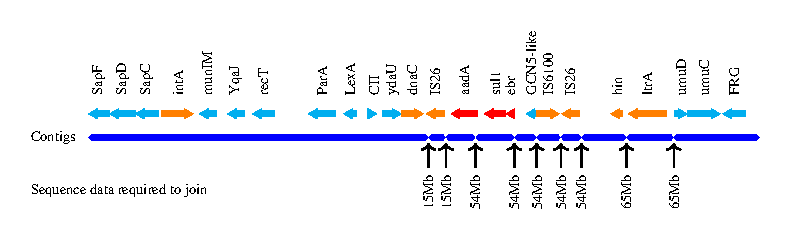
\includegraphics[width=\linewidth]{npscarf/figures/figure3.pdf}
\caption[Structure of a pathogenic island from \kp{}
ATCC BAA-2146]
{Structure of a pathogenic island from \kp{} ATCC BAA-2146. The island harbours three antibiotic resistance genes \emph{strep}, \emph{sul1} and \emph{ebr}, flanked by mobility genes integrase (\emph{int}), inverstase (\emph{hin}), DNA replication (\emph{dnaC}), and insertion sequences (IS26 and IS6100). The island was fragmented into 10 contigs in the Illumina assembly, and was completely resolved with $65$Mbp out of the total of $185$Mbp of nanopore sequence data.}
\label{F:gi}
\end{figure*}


\begin{table*}[!htb]
\centering
\caption{Timeline of determining plasmid-encoded antibiotic resistance genes}
\label{T:plasmidGenes}
\vspace{5pt}
\resizebox{\textwidth}{!}{
\begin{tabular}{cllll}
 \toprule
 Data \\
 required & Gene ID & NCBI ref & Antibiotic resistance & Plasmid evidence\\
\hline
$10$Mbp & blaTEM-1B & JF910132 & penicillins, some cephalosporins & IncR;IncFIA(HI1) \\
      & strB & M96392 & streptomycin & IncR;IncFIA(HI1) \\
      & strA & AF321551 & streptomycin & IncR;IncFIA(HI1) \\     
      & sul2 & GQ421466 & sulfonamides & IncR;IncFIA(HI1) \\
$14$Mbp & aac6Ib & M21682 & tobramycin, amikacin, netilmicin, sisomicin & IncR;IncFIA(HI1) \\
$21$Mbp & mphA & D16251 & erythromycin & IncFIB(K);IncFII(K) \\ 
      & tetA & AJ517790 & tetracyclines & IncFIB(K);IncFII(K) \\
      & QnrB7 & EU043311 & quinolones & IncR;IncFIA(HI1) \\
$29$Mbp & dfrA14 & DQ388123 & trimethoprim & IncR;IncFIA(HI1) \\ 
$46$Mbp &  blaNDM-1 & FN396876 & penicillins, cephalosporins, carbapenems & IncA/C2 \\
$51$Mbp & rmtC & AB194779 & aminoglycosides (include gentamicin, kanamycin) & IncA/C2 \\
$78$Mbp & sul1 & AY224185 & sulphonamide & IncA/C2 \\
      & aac6Ib\_1 & M21682 & tobramycin, amikacin, netilmicin, sisomicin &
      IncA/C2 \\
      & blaCMY-6 & AJ011293 & penicillins, some cephalosporins & IncA/C2\\
$83$Mbp & blaSHV-11 & GQ407109 & penicillins, some cephalosporins &  IncR;IncFIA(HI1) \\ 
      & aac6Ib & M21682 & tobramycin, amikacin, netilmicin, sisomicin &
 IncR;IncFIA(HI1) \\
      & blaOXA-1 & J02967 & penicillins & IncR;IncFIA(HI1) \\
      & aac3-IIa & X51534 & gentamicin, tobramycin, netilmicin, sisomicin &
 IncR;IncFIA(HI1) \\
     
\hline
\end{tabular}
}
\end{table*}

The ability to complete genome assemblies in streaming fashion also enables
real-time analyses that rely on positional information. Such analyses include
identifying genes encoded in bacterial genomic islands and plasmids. These
functional regions in the bacterial genomes can be horizontally transferred
between organisms, which is one of the main mechanisms for acquiring AMR in
pathogenic bacteria. Here we demonstrate these analyses on the multi-drug
resistant \kp{} ATCC BAA-2146 strain.

Prior to scaffolding the Illumina assembly of the sample, we annotated the
assembly using Prokka~\cite{Seemann2014} to identify the positions of genes and
insertion sequences in the assembly. Bacterial genomic islands are genomic
regions longer than $8$Kbp, containing certain classes of genes such as AMR genes.
In addition, they often carry mobility genes such as transposase, integrase and
insertion sequences (IS)~\cite{LangilleHB2010}. These sequences generally
appear multiple times in the genomes (repetitive sequences), causing genomic
islands fragmented in the short read assembly. We ran Islander~\cite{MantriW2004}
and PHAST~\cite{ZhouLL2011} on the Illumina assembly, which together detected
six genomic islands. In the annotation, we also found 28 insertion sequences; 14
of these were within $3$Kbp of the contig ends, suggesting that any genomic
islands flanked by these insertion sequences were fragmented. During scaffolding
of the assembly with nanopore sequencing data, \npscarf{} constructed four
additional genomic islands, which were not previously reported by Islander and
PHAST (data not shown). All 10 genomic islands were precisely in agreement with 
the analysis of the PacBio assembly by~\cite{HudsonBM2014}. Figure~\ref{F:gi}
presents the structure of such a genomic island, namely Kpn23SapB, and the
timeline of its reconstruction. The genomic island harboured three AMR genes, 
namely \emph{aadA} (mediates resistance to streptomycin and spectinomycin), 
\emph{sul1} (sulfonamides) and \emph{ebr} (ethidium bromide and quaternary
ammonium). The genomic island also carried two copies of the insertion sequence 
IS26, which flanked the AMR genes, and a copy of the insertion sequence IS6100.
The presence of these repetitive sequences caused the island to be fragmented 
into 10 contigs in the Illumina assembly; the three resistance genes were in two
different contigs. \npscarf{} required $64.59$Mbp of data (14-fold coverage of the 
genome) to report the full structure of the island (Figure~\ref{F:gi}).


For real-time detection of plasmid-encoded genes, we identified plasmid origin
of replication sequences from the Illumina assembly using the PlasmidFinder
database~\cite{CarattoliZG2014}. Contigs containing a plasmid origin of
replication sequence were considered to be part of a plasmid. Essentially, only 166
genes contained within these contigs could be ascertained as plasmid-encoded 
genes from the Illumina sequencing of the \kp{} ATCC BAA-2146 strain. During 
scaffolding of the Illumina assembly, once a contig was added to a plasmid,
\npscarf{} reported genes in the contig as plasmid-encode genes. The amount of 
long-read sequence data required to assign each gene to a plasmid is presented in 
the Supplementary Spreadsheet.  

With the Illumina assembly, we identified 27 AMR genes,  but none was in a
contig containing a plasmid origin replication sequence. As such, whether any 
of these genes were carried by a plasmid could only be ascertained with long
reads. Table~\ref{T:plasmidGenes} presents the time-line of such determination.
In particular, we confirmed 18 AMR genes as plasmid-encoded with $83$Mbp
($\sim$14-fold coverage) of nanopore sequencing data. In addition, as all four
plasmids were circularised and complete with $103$Mbp ($\sim$18-fold coverage) of
data, we could confidently conclude that only these 18 AMR genes were
plasmid-encoded, even before the completion of the full genome assembly and the
sequencing run.

\subsection{Comparison with other methods}

\newcommand{\cthead}[2]{\multicolumn{#1}{c}{\textbf{#2}}}
\LTcapwidth=\linewidth
\footnotesize
\begin{longtable}{llcrrrrr@{\hspace{2pt}}c@{\hspace{2pt}}r}
\caption{Comparison of assemblies produced by \npscarf{} and the comparative methods} \label{T:compare} \\

 \toprule
    &       & \cthead{1}{Assembly} & \cthead{1}{\#Contigs}      & 
    \cthead{1}{N50}  & \cthead{1}{Mis-} &  \cthead{1}{Error}  &
    \cthead{3}{Run times} \\
    & \cthead{1}{Method} & \cthead{1}{size (Mbp)} &\cthead{1}{($\geq500$bp)} &
    \cthead{1}{(Kp)} & \cthead{1}{assemblies} & \cthead{1}{(per $100$Kbp)} &  
    \cthead{3}{(CPU hrs)} \\
\toprule    
\endfirsthead

\multicolumn{10}{c}%
{{\tablename\ \thetable{} -- continued from previous page}} \\
 \toprule
    &       & \cthead{1}{Assembly} & \cthead{1}{\#Contigs}      & 
    \cthead{1}{N50}  & \cthead{1}{Mis-} &  \cthead{1}{Error}  &
    \cthead{3}{Run times} \\
    & \cthead{1}{Method} & \cthead{1}{size (Mbp)} &\cthead{1}{($\geq500$bp)} &
    \cthead{1}{(Kp)} & \cthead{1}{assemblies} & \cthead{1}{(per $100$Kbp)} &  
    \cthead{3}{(CPU hrs)} \\
\toprule    
\endhead

\hline \multicolumn{10}{|r|}{{Continued on next page}} \\ \hline
\endfoot

\hline \hline
\endlastfoot

\rowcolor{Gray} \multicolumn{10}{l}
{ \kp{} ATCC BAA-2146. Nanopore data: 33X coverage} \\  
 & SPAdes & 5.70 & 90 & 288 & 0 & 4.72 & 15.63 &  & \\
 & SPAdes-Hybrid & 5.75 & 17 & 3,076 & 1 & 6.61 & 16.07 &  & \\
 & SPAdes+SSPACE & 5.74 & 53 & 400 & 4 & 12.73 & 15.63 & + & 2.3 \\
 & SPAdes+LINK & 5.74 & 31 & 554 & 5 & 16.05 & 15.63 & + & 4.03 \\
 & SPAdes+\npscarf{} (rt)& 5.78 & 5 & 5,438 & 0 & 20.00 & 15.63 & + & 1.6 \\
 & SPAdes+\npscarf{} (b) & 5.78 & 5 & 5,438 & 0 & 22.76 & 15.63 & + & 0.84 \\
 & NaS+CA & 5.89 & 29 & 345 & 15 & 18.89 & 324.35 & + & 3.49 \\
 & Nanocorr+CA & 5.68 & 68 & 139 & 8 & 141.32 & 312.64 & + & 1.37 \\
 & Canu+Pilon & 0 &  -  &  -  &  -  &  -  &  -  &  &  -  \\
 & Miniasm+Pilon & 0 &  -  &  -  &  -  &  -  &  -  &  &  -  \\
\rowcolor{Gray} \multicolumn{10}{l}
{\kp{} ATCC 13883. Nanopore data:  18X coverage} \\ 
 & SPAdes & 5.51 & 69 & 302 & 5 & 6.22 & 16.95 &  & \\
 & SPAdes-Hybrid & 5.54 & 15 & 729 & 19 & 8.02 & 16.97 &  & \\
 & SPAdes+SSPACE & 5.55 & 36 & 685 & 13 & 12.39 & 16.95 & + & 1.48 \\
 & SPAdes+LINK & 5.55 & 17 & 1,527 & 18 & 16.12 & 16.95 & + & 1.12 \\
 & SPAdes+\npscarf{} (rt) & 5.55 & 4 & 4,924 & 21 & 10.84 & 16.95 & + & 0.52
 \\
 & SPAdes+\npscarf{} (b) & 5.55 & 4 & 4,924 & 21 & 10.26 & 16.95 & + & 0.45 \\
 & NaS+CA & 5.46 & 38 & 394 & 36 & 10.24 & 192.78 & + & 6.92 \\
 & Nanocorr+CA & 5.02 & 60 & 148 & 16 & 118.34 & 161.33 & + & 2.6 \\
 & Canu+Pilon & 0.04 & 4 & 12 & 4 & 10.40 & 0.53 & + & 0.46 \\
 & Miniasm+Pilon & 0.03 & 3 & 13 & 1 & 14.12 & 0.00 & + & 0.26 \\
\rowcolor{Gray} \multicolumn{10}{l}
{ \ec{} K12 MG1655. Nanopore data: 67X coverage} \\
 & SPAdes & 4.61 & 114 & 176 & 0 & 3.51 & 4.38 &  & \\
 & SPAdes-Hybrid & 4.67 & 42 & 4,643 & 2 & 1.21 & 4.76 &  & \\
 & SPAdes+SSPACE & 4.66 & 59 & 3,155 & 1 & 29.26 & 4.38 & + & 3.42 \\
 & SPAdes+LINK & 4.66 & 50 & 3,318 & 2 & 36.19 & 4.38 & + & 4.03 \\
 & SPAdes+\npscarf{} (rt) & 4.64 & 1 & 4,644 & 2 & 13.08 & 4.38 & + & 2.43 \\
 & SPAdes+\npscarf{} (b) & 4.64 & 1 & 4,646 & 2 & 11.72 & 4.38 & + & 1.91 \\
 & NaS+CA & 4.87 & 21 & 874 & 19 & 10.60 & 807.19 & + & 6.77 \\
 & Nanocorr+CA & 4.66 & 2 & 4,650 & 6 & 10.41 & 213.68 & + & 8.49 \\
 & Canu+Pilon & 0.11 & 9 & 14 & 0 & 13.90 & 0.79 & + & 0.28 \\
 & Miniasm+Pilon & 1.91 & 85 & 23 & 1 & 595.61 & 0.04 & + & 1.24 \\
\rowcolor{Gray} \multicolumn{10}{l}
{S. Typhi H58. Nanopore data:  26X coverage}\\ 
 & SPAdes & 4.84 & 89 & 107 & 7 & 39.05 & 1.86 &  & \\
 & SPAdes-Hybrid & 4.88 & 27 & 443 & 12 & 55.46 & 2.06 &  & \\
 & SPAdes+SSPACE & 4.88 & 34 & 358 & 10 & 59.39 & 1.86 & + & 1.55 \\
 & SPAdes+LINK & 4.86 & 20 & 473 & 13 & 66.65 & 1.86 & + & 1.28 \\
 & SPAdes+\npscarf{} (rt) & 4.87 & 9 & 864 & 18 & 53.86 & 1.86 & + & 0.93 \\
 & SPAdes+\npscarf{} (b) & 4.86 & 8 & 864 & 16 & 52.01 & 1.86 & + & 0.47 \\
 & NaS+CA & 4.97 & 54 & 212 & 17 & 58.87 & 248.32 & + & 7.21 \\
 & Nanocorr+CA & 2.98 & 95 & 37 & 9 & 973.63 & 199.85 & + & 0.94 \\
 & Canu+Pilon & 0 &  -  &  -  &  -  &  -  &  -  &  &  -  \\
 & Miniasm+Pilon & 0.02 & 2 & 14 & 0 & 10.96 & 0.01 & + & 0.26 \\
\rowcolor{Gray} \multicolumn{10}{l}
{ \sce{} W303. Nanopore data: 196X coverage}\\ 
 & SPAdes & 11.82 & 364 & 155 & 29 & 124.10 & 20.54 &  & \\
 & SPAdes-Hybrid & 12.06 & 240 & 346 & 68 & 158.13 & 67.81 &  & \\
 & SPAdes+SSPACE & 13.39 & 263 & 392 & 89 & 136.66 & 20.54 & + & 31.54 \\
 & SPAdes+LINK & 12.09 & 161 & 580 & 83 & 143.04 & 20.54 & + & 26.97 \\
 & SPAdes+\npscarf{} (rt) & 12.00 & 19 & 913 & 82 & 141.93 & 20.54 &
 + & 21.28 \\
 & SPAdes+\npscarf{} (b) & 11.90 & 17 & 924 & 79 & 141.01 & 20.54 & + &
 18.84 \\
 & NaS+CA & 12.76 & 121 & 155 & 123 & 140.08 & 9811.88 & + & 140.69 \\
 & Nanocorr+CA & 13.48 & 108 & 600 & 133 & 197.00 & 7208.08 & + & 272.86
 \\
 & Canu+Pilon & 12.31 & 43 & 497 & 81 & 229.08 & 599.36 & + & 58.5 \\
 & Miniasm+Pilon & 11.79 & 51 & 391 & 41 & 1400.82 & 0.27 & + & 30.27 \\
\end{longtable}

\normalsize

We compared the performance of our algorithm against existing methods that were
reported to build assemblies with nanopore sequencing. In addition to the two
samples presented above, we sourced three other samples reported in the
literature including \emph{i}.) an \emph{Escherichia coli} K12 MG1655
strain sequenced to 67-fold coverage with a nanopore R7.3 flowcell and standard
library preparation~\cite{QuickQL2014}; \emph{ii}.) a \emph{Salmonella
enterica} serovar Typhi (S. Typhi) haplotype, H58~\cite{AshtonND2015} sequenced to
27-fold and \emph{iii}.) a \emph{Saccharomyces cerevisiae} W303 genome
(196-fold)~\cite{GoodwinGE2015}.
Note that the coverage reported here was from all base-called data (including
both 1D and 2D reads). Of the methods selected for comparison,
SPAdes-hybrid~\cite{BankevichNA2012}, SSPACE-LongRead~\cite{BoetzerP2014},
LINKS~\cite{WarrenYV2015} and \npscarf{} were scaffolders, whereas
Nanocorr~\cite{GoodwinGE2015} and NaS~\cite{MadouiEC2015} belonged to the
error correction category. We assembled the Illumina data of these samples using
SPAdes~\cite{BankevichNA2012} before running the scaffolding methods with
nanopore data. SPAdes-hybrid was run by incorporating nanopore data into the
assembly (with --nanopore option). The two error correction tools Nanocorr and
NaS were run on the nanopore sequencing data using about 50-fold coverage of
Illumina data, as suggested by authors of the respective publications. The corrected
reads were then assembled using Celera Assembler~\cite{MyersSD2000}. We
observed that the quality of the assemblies produced by Celera Assembler were
highly sensitive to the parameters specified in the specification file. We
therefore ran Celera Assembler for each dataset on three specification files
provided by the authors of NaS and Nanocorr, and report here the most complete
assembly obtained.
We also ran two popular \emph{de novo} assembly methods,
Canu~\cite{BerlinKC2015} and Miniasm~\cite{Li2016} on these datasets.
These methods necessitated a polishing step using Pilon~\cite{WalkerAS2014}.


We evaluated the assemblies in terms both of completeness and accuracy.
The completeness of an assembly was assessed by N50 statistics and the
number of contigs that were longer than 500 bp. To examine the accuracy of an
assembly, we compared it with the closest reference genome of the samples in
NCBI (See Methods) to obtain the number of misassemblies, mismatches and
short indels.
During the test, we recorded the CPU times
required by these pipelines to produce the assemblies. Run times for
the scaffolder methods included times for running SPAdes and for scaffolding,
while those for NaS and Nanocorr included correction time and Celera
Assembler time.
The times reported for the \emph{de novo} methods included that for
polishing using Pilon.
Table~\ref{T:compare} presents the comparison metrics of all assemblies as 
reported by Quast~\cite{GurevichSV2013}, as well as their run times. 
 
We ran \npscarf{} in real-time mode, in which nanopore sequencing data are
streamed to the pipeline in the exact order they were generated.
This allowed us to assess the completeness of the assemblies against the 
amount of data generated.
Figure~\ref{f:scaffold} shows the progress of completing the assemblies
for all five samples. As mentioned previously, \npscarf{} produced complete and
near-complete assemblies for the two \kp{} samples (Figures~\ref{f:scaffold}a
and \ref{f:scaffold}b) with under 20-fold coverage of nanopore data.
For the \ec{} K12 MG1655 sample, \npscarf{} required less than 30-fold coverage of 
nanopore data to complete the genome assembly with one circular contig.
\npscarf{} also reduced the S. Typhi assembly to only nine contigs (N50=$864$Kbp),
which was significantly better than the assembly reported by~\cite{AshtonND2015} 
from the same data (34 contigs, N50=$319$Kbp).

As for the \sce{} W303 genome, which contains 16 nuclear chromosomes and one 
mitochondrial chromosome, \npscarf{} generated an assembly of 19 contigs (N50=$913$Kbp); 
substantially fewer than 
the 108 contigs (N50=$600$Kbp) generated by the next best method (Nanocorr, 
see Table~\ref{T:compare}).
We noticed a drop in N50 statistics at the point where about 50-fold coverage 
of nanopore data were received (Figure~\ref{f:scaffold}e). This was because
\npscarf{} encountered contradicting bridges and hence broke the assembly at 
the lowest scoring bridge in lieu of a higher scoring one. The N50 was then 
improved to reach the N50 of $913$Kbp with 90-fold coverage of nanopore sequencing; 
the assembly did not change with more data (90-fold to 196-fold). 
We examined the assembly by comparing that with the reference genome of \sce{}
strain S288C. One of the contigs (Contig 17,
length = $81$Kbp) was reported to be circular, which was completely aligned to the 
mitochondrial chromosome of the reference genome. Ten chromosomes (II,
IV, V, VII, IX, X, XI, XIII, XV and XVI) were completely assembled into individual
contigs, and three chromosomes (I, III and VIII) were assembled into two contigs per 
chromosome (See Supplementary Figure 3). We found a misassembly that joined
chromosome IV and the start of chromosome XIV into Contig 10. The end of
chromosome XIV was also joined with chromosome XII into Contig 2. These
misassemblies essentially fused these three chromosomes into two contigs.
We found these mis-assemblies were due to the presence of interspersed repeat
elements which are known for being problematic in assembly
analysis~\cite{TreangenS2012}. The assemblies produced by Canu and Miniasm also
presented several mis-assemblies fusing different chromosomes together, 
emphasising the challenges posed by interspersed repeats in assembling complex 
genomes (See Supplementary Figures 4 and 5).


We reran \npscarf{} on the datasets in batch mode, in which the scaffolding was
performed with the complete dataset. We found that all five assemblies were  
more complete than in real-time mode. In particular, the \sce{} W303
assembly was further reduced to 17 contigs as chromosomes I and VIII were 
resolved into individual contigs (data not shown). In this assembly, 12 out of
17 chromosomes were completely recovered to one contig, one chromosome (XIII)
was fragmented into two contigs and three chromosomes were fused into two
contigs due to misassemblies


In all datasets, \npscarf{} consistently
produced the most complete assemblies, while its accuracy was among the best.
It was the only method that was able to completely resolve the \kp{} ATCC BAA-2146
genome (five contigs, N50 of $5.4$Mbp) with no misassembly, requiring only
20-fold coverage of nanopore data; the second most completed assembly 
(produced by SPAdes Hybrid) contained 17 contigs and had the N50 of 
only $3.1$Mbp despite using 33-fold coverage of nanopore sequence data.
On the well studied \ec{} K12 MG1655 strain
sample where LINK, NaS and Nanocorr were reported to resolve the whole genome
with a larger dataset (147-fold coverage)~\cite{WarrenYV2015}, 
none of these methods could produce the same result on the 67-fold coverage data
set we tested. On the other hand, \npscarf{} was able to reconstruct the genome
into one circular contig with as little as 30-fold coverage of the 
data. On the S. Typhi dataset, \npscarf{} produced assemblies with nine contigs
in real-time mode, and with eight contigs in batch mode (N50=$864$Kbp),
significantly better than assemblies from other methods (over 20 contigs).
We observed that the \emph{de novo} methods, Canu and Miniasm failed to
construct a skeleton for the these bacterial genomes (either no output or only 
a few small sequences produced), possibly due to the low coverage of these
datasets.


The \sce{} W303 assembly produced by \npscarf{} was near complete and N50
statistics reached the theoretical limit of $924$Kbp. Note that \npscarf{} obtained
these results from only less than half of the dataset (95-fold coverage). On
the whole dataset (196-fold coverage), Canu and Miniasm produced assemblies of
43 contigs (N50=$496$Kbp) and 51 contigs (N50=$391$Kbp), respectively. These
assemblies contained more than twice as many contigs as the results from
\npscarf{}. The second most complete assembly in terms of N50 statistic was
produced by Nanocorr (N50=$600$Kbp) which was significantly lower than that from
\npscarf{}.


We observed that the scaffolding methods and the
\emph{de novo} methods were much faster than the error correction counterparts.
Both NaS and Nanocorr 
required the alignment of the short reads to the long reads, which were
computationally expensive. On the other hand, the scaffolding pipelines
required 20 CPU hours or less to build an assembly from short reads,
and from a few hours to around 30 hours to scaffold the assembly with long 
reads. 
As Canu and Miniasm did not produce a decent assembly for the bacterial data 
sets, we only include them in the comparison for the \sce{} dataset. Miniasm
was the fastest on this dataset, requiring only 0.27 CPU-hours to assemble and
over 30 CPU-hours to polish the genome.
Apart from SPAdes-Hybrid, which performed scaffolding as part of short read
assembly, \npscarf{} was the fastest among other scaffolders and consistently required
less scaffolding time. Note that the times reported in Table~\ref{T:compare}
were for processing the entire nanopore dataset, whereas \npscarf{} could be
terminated early once a desirable assembly was obtained.
We observed that \npscarf{} required only 2GB of memory for scaffolding
the bacterial datasets, and 4GB for the \sce{} dataset, which can be easily
installed on a laptop computer. A summary of memory usage of other tools was
presented in Supplementary Table 1.

 
\section{Discussion}

The development of high-throughput long read sequencing technologies such as 
PacBio and nanopore has opened up opportunities for resolving repetitive 
sequences to assemble complete genomes and to improve existing genome assemblies.
However, the relatively high error rates of these technologies pose a challenge
to the accurate assembly of genome sequences. 
An obvious solution is to combine long and erroneous reads with more
accurate and cheaper short read data for assembling genomes~\cite{KorenSW2012,
BashirKR2013}. 
One such approach is to perform \emph{de novo} assembly of long
reads to generate a skeleton of the genome, and error correct the skeleton with
accurate short reads~\cite{BerlinKC2015, Li2016}. Alternatively, erroneous
long reads are corrected~\cite{KorenSW2012, BashirKR2013, GoodwinGE2015,
MadouiEC2015} before being assembled with classical assemblers designed for long
and accurate reads such as Celera Assembler~\cite{MyersSD2000}.
These approaches usually require large amounts of long read data.
Hybrid assemblers in the scaffolding class harness long spanning reads to guide
the extension of contigs in the draft genome assemblies. For example,
SSPACE-LongRead~\cite{BoetzerP2014} and Cerulean~\cite{DeshpandeFP2013} rely
on the alignment of long reads to the assembly graph to determine the adjacent
contigs. LINKS~\cite{WarrenYV2015} uses a k-mer approach, which further
improves the running time with a small sacrifice of accuracy.
Overall, hybrid-assembly methods, especially those in the scaffolding category,
provide economical genome finishing pipelines that can produce high quality
genome assemblies from small amounts of long read data on modest computing 
equipment.
\npscarf{} is similar to these mentioned scaffolders in the sense that it aligns
the long reads to the contigs to build a scaffold of the genome.
However, our method estimates the copy number
of each contig in the genome and constructs the scaffold from non-repetitive 
contigs, while the repetitive contigs are used to fill the gaps in the scaffold.
Consequently, we demonstrated that \npscarf{} is capable of generating more
complete and accurate assemblies than the competitors, while requiring much
less data.

 

To date, there is no prominent assembler that takes advantage of the
real-time feature from nanopore sequencing. Nanopore technology allows one to 
terminate a run and wash the flowcell for
subsequent runs without compromising sequencing yield and quality.
The ability to analyse data on the fly and to stop a sequencing run when
sufficient data are generated plays a critical role to control resources
necessary for a single experiment.

One of the main contributions of our algorithm is that it can process data
streaming from the sequencer and report the current status of the analysis in
real-time. 
Our pipeline still relies on a base-caller, and the introduction of
fast real-time base-callers such as Nanocall~\cite{DavidDY2016} and
DeepNano~\cite{BozaBV2016} helps to reduce the latency. 
The current pipeline processes a sequence read within minutes 
of it finishing traversing the pore, rather than as the read is actually passing 
through the pore, and as such is real-time at the temporal resolution of minutes, 
but not at the millisecond level required to update with the addition of each 
base. However, this temporal resolution is sufficient to allow our pipeline 
to answer the biological problems at hand 
at the earliest possible time, and while sequencing is still in progress.
Investigators can also assess the progress of the analysis, and terminate 
the sequencing once an assembly of sufficient quality and completeness is
obtained. This enables the generation of sufficient data necessary for the 
analysis to guarantee the experimental outcomes and, at the same time, avoids
costly over-sequencing. 
While our pipeline still requires short read data which cannot
be generated in real-time with current technology, it offers a strategy to
minimise the generation of the more expensive long read data.


The real-time function to complete genomic sequences opens the possibility of
\emph{in situ} biological analyses \cite{CaoGE2016}. Certain biological markers
of interest may be identified from short read assemblies, but their positions in
the genome could only be determined by completing the genome assembly with long
reads. We have shown that \npscarf{} can facilitate such analyses in real-time by
demonstrating the identification of AMR genes encoded in
plasmids and pathogenicity islands.


\section{Methods}

\subsection{Determining unique contigs}
Before scaffolding a fragmented short read genome assembly, \npscarf{}
determines the multiplicity of each contig in the assembly by comparing short
read sequencing coverage of the contig to that of the whole genome. Coverage
information is often included in the sequences assembled by most tools, such as
SPAdes~\cite{BankevichNA2012} and Velvet~\cite{Zerbino2008}, or can otherwise 
be obtained from the mapping of short reads to the assembly. 
An reasonable estimate for depth coverage of the genome is that of the largest
contig. \npscarf{} however leverages this to the \emph{normalised average
coverage} of the largest contigs so long as their depth coverage does not
deviate from the estimated genome depth coverage.
More formally, let $depth_i$ and $len_i$ respectively represent the sequencing
depth (coverage) and the length of contig $i$, where contigs are sorted in
decreasing order in length. Let $depth_g$ represent the estimated coverage
of the whole genome. \npscarf{} first initialises $depth_g$ to that of the
largest contig:
\begin{equation}\label{E:depth}
depth_g^1 = depth_1
\end{equation}
It then iteratively updates the estimate   
\begin{equation}\label{E:gdepth}
depth_g^i = \dfrac{\sum_i depth_i \times len_i}{\sum_i len_i} 
\end{equation}
and terminates the process when the depth coverage of the next contig greater
than a threshold
\begin{equation}\label{E:cov}
\dfrac{depth_i}{depth_g^{i-1}} > \theta
\end{equation}
\npscarf{} set the threshold $\theta$ to 1.5. In our experience, the statistic is
stable with up to 20 of the largest contigs longer than $20$Kbp, which are most
likely unique contigs in bacterial genomes ~\cite{KorenP2015}. We hence also
add these into the condition for termination.
The multiplicity of contig $i$ ($mul_i$) is determined by
\begin{equation}\label{E:mul}
mul_i= \dfrac{depth_i}{depth_g}
\end{equation}
\npscarf{} considers a contig unique if its multiplicity is less than $\theta$.
 

\subsection{Bridging unique contigs and filling gaps with repetitive contigs}
\npscarf{} next builds the backbone of the genome from the unique contigs.
It identifies the long reads that are aligned to two unique contigs, thereby
establishing the relative position (\IE, distance and orientation) of these
contigs. To minimise the effect of false positives that can arise from
aligning noisy long reads, \npscarf{} groups reads that consistently support
a particular relative position into a bridge and assigns the bridge 
a score based on the number of supporting reads and the alignment quality of
these reads. When two unique contigs are connected by a bridge, they are merged
into one larger unique contig. \npscarf{} uses a greedy strategy based on 
Kruskal's algorithm~\cite{Kruskal1956}, which merges contigs from the highest
scoring bridges. In the newly created contig, the gap is temporarily filled with
the consensus sequence of the reads forming the bridge. \npscarf{} then identifies
repetitive contigs that are aligned to this consensus sequence, and uses these
contigs to fill in the gap.


\subsection{Real-time processing}
To support real-time analysis of nanopore sequencing, the previously described
algorithm can be augmented to process long read data directly from a stream
(See Figure~\ref{f:workflow}).
In this mode, \npscarf{} employs a mapping method that supports streaming
processing such as BWA-MEM~\cite{Li2013} to align a small number of long reads
to the existing assembly as they arrive. This block-wise processing allows
\npscarf{} to make use of information from a small batch of reads sequenced
within a short period of time (within minutes). If a read is aligned to two
unique contigs, it is added to the bridge connecting the two contigs. Once the bridge
reaches a pre-defined scoring threshold,
the two contigs are merged and the gap is filled as above. 
In case this merging contradicts with the existing assembly (for example, if the
relative distance and/or orientation implied by the bridge is inconsistent with 
those of previously used bridges) \npscarf{} revisits the previous bridges, breaks
the smallest scoring contradicting bridge and uses the current bridge instead. 
The algorithm hence gradually improves the completeness and the quality of the 
assembly as more data are received.

\subsection{Bacterial cultures and DNA extraction}
Bacterial strains \kp{} ATCC BAA-2146 ( (NDM-1 positive) and ATCC 13883
(type strain) were obtained from American Type Culture Collection (ATCC, USA).
Bacterial cultures were grown overnight from a single colony at 37 $^{\circ}$C
with shaking (180 rpm). Whole cell DNA was extracted from the cultures using the DNeasy Blood and Tissue Kit
(QIAGEN$\copyright$, Cat \#69504) according to the bacterial DNA extraction
protocol with modified enzymatic lysis pre-treatment.

\subsection{Illumina sequencing and assembly} 
Library preparation was performed using the NexteraXT DNA Sample preparation kit 
(Illumina), as recommended by the manufacturer. Libraries were sequenced on the 
MiSeq instrument (Illumina) with 300 bp paired end sequencing, to a coverage of
over 250-fold. 

\subsection{MinION sequencing}
Library preparation was performed using the Genomic DNA Sequencing kit 
(Oxford Nanopore), according to the manufacturer's instructions. 
For the R7 MinION Flow Cells SQK-MAP-002 sequencing kit was used and for 
R7.3 MinION Flow Cells SQK-MAP-003 were used, according to the manufacturer's
instructions. A new MinION Flow Cell (R7 or R7.3) was used for each sequencing run. 
The library was loaded onto the MinION Flow Cell and the 
Genomic DNA 48-hour sequencing protocol was initiated using MinKNOW software.


\subsection{Data collection}
MinION data for the \ec{} K12 MG1655 sample~\cite{LomanQ2014} were downloaded
from the European Nucleotide Archive (ENA) with accession number ERP007108. We used the
data from the chemistry R7.3 run (67-fold coverage of the genome from run
accession ERR637419) rather than the chemistry R7 reported in work
by~\cite{GoodwinGE2015, WarrenYV2015, MadouiEC2015}. Illumina MiSeq sequencing
data for the sample were also obtained from ENA (assession number ERR654977). 
Data from both Illumina and MinION sequencing of the S. Typhi 
strain~\cite{AshtonND2015} were collected from ENA
accession number ERP008615. The \sce{} W303 sequencing data were
provided by~\cite{GoodwinGE2015} from the website
\url{http://schatzlab.cshl.edu/data/nanocorr/}.


\subsection{Data processing}
Read data from Illumina sequencing were trimmed with \emph{trimmomatic}
V0.32~\cite{BolgerLU2014} and subsequently assembled using SPAdes
V3.5~\cite{BankevichNA2012}. SPAdes was run with the recommended parameters (-k
21,33,55,77,99,127 --careful). SPAdes-Hybrid was run with the inclusion of the
--nanopore option. SSPACE and LINKS were run on the original SPAdes' assemblies.
For SSPACE, we used the parameters reported to work with MinION reads
in~\cite{KarlssonLS2015} (-i 70 -a 1500 -g -5000). In the case of LINKS, a script
was adapted from the example run for \ec{} K12 MG1655 sample to allow 30
iterations of the algorithms being executed for each dataset. NaS and Nanocorr
were applied to correct nanopore data from the maximum of 50-fold coverage of
Illumina data. The corrected long reads were assembled using Celera Assembler
version 8.3 with the configuration files provided by the respective publication.
Canu was run with the recommended parameter for nanopore data 
(-nanopore-raw). Miniasm were run with its default parameter. The short reads 
were aligned to Canu's and Miniasm's assemblies by BWA-MEM, and Pilon was run on 
the alignments to polish the assembly sequences.


The Illumina assembly of \kp{} ATCC BAA-2146 was annotated using 
Prokka (version 1.12-beta) with the recommended parameters for a \kp{} strain.
AMR genes from the assembly were identified using the ResFinder 
database~\cite{ZankariHC2012}.
Plasmid origin of replication sequences in both \kp{} assemblies were identified 
by uploading the assembly to the PlasmidFinder database~\cite{CarattoliZG2014}.


In real-time analysis, \npscarf{} aligned incoming long
reads using BWA-MEM~\cite{Li2013} with the parameters --k11 --W20 --r10
--A1 --B1 --O1 --E1 --L0 --a --Y --K10000 . The --K10000 parameter allowed 
alignments to be streamed to the scaffolding algorithm after several reads 
were aligned. 

\subsection{Comparative metrics}
The assemblies produced by the mentioned methods were evaluated using Quast
(V3.2) to compare with the respective reference sequences. The number of contigs,
N50 statistics and the number of misassemblies were as per Quast reports.
The error rates were computed from sum of the number of mismatches and the indel
length. The CPU time for each pipeline was measured using the Linux time command 
(/usr/bin/time -v); the sum of user time and system time was reported. 
When a pipeline was distributed across a computing cluster, its CPU time was the
sum of that across all jobs.

\subsection{Data availability}
Sequencing data for the two \kp{} samples were deposited to the
European Nucleotide Archive (ENA). The accession numbers for the MinION sequencing data are
ERR1474979 and ERR1474981, and that for the MiSeq sequencing data are 
ERR1474547 and ERR1474549.
The software presented in this article and its documentation is publicly
available at GitHub \url{https://github.com/mdcao/npScarf}.


%\section{Authors' contributions}
%MDC and LC conceived the study. SN, MDC and LC designed and implemented 
%the algorithm. AE performed the bacterial cultures and DNA extractions. 
%DG performed the MinION sequencing and Illumina sequencing. SN and MDC 
%performed the analysis and wrote the first draft of the manuscript. 
%All authors contributed to editing the final manuscript.
%
%\section{Competing financial interests}
%MC is a participant of Oxford Nanopore's MinION Access Programme (MAP) and 
%received the MinION device, MinION Flow Cells and Oxford Nanopore Sequencing 
%Kits in return for an early access fee deposit. MDC received travel and
%accommodation expenses to speak at an Oxford Nanopore-organised conference.
%None of the authors have any commercial or financial interest in Oxford
%Nanopore Technologies Ltd.
%
%\section{Acknowledgements}
%MAC is an National Health and Medical Research Council Principal Research Fellow (APP1059354). LC is an Australian Research Council Future
%Fellow (FT110100972). The research is supported by funding from the National Health and Medical Research Council (APP1052303) as well as funding from the 
%Institute for Molecular Bioscience Centre for Superbugs Solutions (610246).

%%%%%%%%%%%%%%%%%%%%%%%%%%%%%%%%%%%%%%%%%%%%%%%%%%%%%%%%%%%%%%%%%%%%%%%%%%%%%%%%%%%%

%\begin{thebibliography}{10}
%\expandafter\ifx\csname url\endcsname\relax
%  \def\url#1{\texttt{#1}}\fi
%\expandafter\ifx\csname urlprefix\endcsname\relax\def\urlprefix{URL }\fi
%\expandafter\ifx\csname doiprefix\endcsname\relax\def\doiprefix{DOI }\fi
%\providecommand{\bibinfo}[2]{#2}
%\providecommand{\eprint}[2][]{\url{#2}}
%
%\bibitem{AshtonND2015}
%\bibinfo{author}{Ashton, P.~M.} \emph{et~al.}
%\newblock \bibinfo{title}{{MinION nanopore sequencing identifies the position
%  and structure of a bacterial antibiotic resistance island}}.
%\newblock \emph{\bibinfo{journal}{Nature Biotechnology}}
%  \textbf{\bibinfo{volume}{33}}, \bibinfo{pages}{296--300}
%  (\bibinfo{year}{2015}).
%\newblock
%\urlprefix\url{http://www.nature.com/nbt/journal/v33/n3/full/nbt.3103.html}.
%\newblock \doiprefix 10.1038/nbt.3103.
%
%\bibitem{KasianowiczBB1996}
%\bibinfo{author}{Kasianowicz, J.~J.}, \bibinfo{author}{Brandin, E.},
%  \bibinfo{author}{Branton, D.} \& \bibinfo{author}{Deamer, D.~W.}
%\newblock \bibinfo{title}{{Characterization of individual polynucleotide
%  molecules using a membrane channel}}.
%\newblock \emph{\bibinfo{journal}{Proceedings of the National Academy of
%  Sciences}} \textbf{\bibinfo{volume}{93}}, \bibinfo{pages}{13770--13773}
%  (\bibinfo{year}{1996}).
%\newblock \urlprefix\url{http://www.pnas.org/content/93/24/13770.full}.
%\newblock \doiprefix 10.1073/pnas.93.24.13770.
%
%\bibitem{BrantonDM2008}
%\bibinfo{author}{Branton, D.} \emph{et~al.}
%\newblock \bibinfo{title}{{The potential and challenges of nanopore
%  sequencing.}}
%\newblock \emph{\bibinfo{journal}{Nature biotechnology}}
%  \textbf{\bibinfo{volume}{26}}, \bibinfo{pages}{1146--53}
%  (\bibinfo{year}{2008}).
%\newblock \doiprefix 10.1038/nbt.1495.
%
%\bibitem{StoddartHM2009}
%\bibinfo{author}{Stoddart, D.}, \bibinfo{author}{Heron, A.~J.},
%  \bibinfo{author}{Mikhailova, E.}, \bibinfo{author}{Maglia, G.} \&
%  \bibinfo{author}{Bayley, H.}
%\newblock \bibinfo{title}{{Single-nucleotide discrimination in immobilized DNA
%  oligonucleotides with a biological nanopore.}}
%\newblock \emph{\bibinfo{journal}{Proceedings of the National Academy of
%  Sciences of the United States of America}} \textbf{\bibinfo{volume}{106}},
%  \bibinfo{pages}{7702--7} (\bibinfo{year}{2009}).
%\newblock \urlprefix\url{http://www.pnas.org/content/106/19/7702.abstract}.
%\newblock \doiprefix 10.1073/pnas.0901054106.
%
%\bibitem{ChinAM2013}
%\bibinfo{author}{Chin, C.-S.} \emph{et~al.}
%\newblock \bibinfo{title}{{Nonhybrid, Finished Microbial Genome Assemblies from
%  Long-Read SMRT Sequencing Data}}.
%\newblock \emph{\bibinfo{journal}{Nature Methods}}
%  \textbf{\bibinfo{volume}{10}}, \bibinfo{pages}{563--569}
%  (\bibinfo{year}{2013}).
%\newblock
%  \urlprefix\url{http://www.nature.com/nmeth/journal/v10/n6/abs/nmeth.2474.html}.
%\newblock \doiprefix 10.1038/nmeth.2474.
%
%\bibitem{LomanQS2015}
%\bibinfo{author}{Loman, N.~J.}, \bibinfo{author}{Quick, J.} \&
%  \bibinfo{author}{Simpson, J.~T.}
%\newblock \bibinfo{title}{{A complete bacterial genome assembled de novo using
%  only nanopore sequencing data}}.
%\newblock \emph{\bibinfo{journal}{Nature Methods}}
%  \textbf{\bibinfo{volume}{12}}, \bibinfo{pages}{733--735}
%  (\bibinfo{year}{2015}).
%\newblock
%\urlprefix\url{http://www.nature.com/nmeth/journal/v12/n8/full/nmeth.3444.html}.
%\newblock \doiprefix 10.1038/nmeth.3444.
%
%\bibitem{BerlinKC2015}
%\bibinfo{author}{Berlin, K.} \emph{et~al.}
%\newblock \bibinfo{title}{{Assembling large genomes with single-molecule
%  sequencing and locality-sensitive hashing}}.
%\newblock \emph{\bibinfo{journal}{Nature Biotechnology}}
%  \textbf{\bibinfo{volume}{33}}, \bibinfo{pages}{623--630}
%  (\bibinfo{year}{2015}).
%\newblock
%  \urlprefix\url{http://www.nature.com/nbt/journal/vaop/ncurrent/abs/nbt.3238.html}.
%\newblock \doiprefix 10.1038/nbt.3238.
%
%\bibitem{Li2016}
%\bibinfo{author}{Li, H.}
%\newblock \bibinfo{title}{{Minimap and miniasm: fast mapping and de novo
%  assembly for noisy long sequences}}.
%\newblock \emph{\bibinfo{journal}{Bioinformatics}}
%  \textbf{\bibinfo{volume}{32}}, \bibinfo{pages}{2103--2110}
%  (\bibinfo{year}{2016}).
%\newblock \urlprefix\url{
%  http://bioinformatics.oxfordjournals.org/lookup/doi/10.1093/bioinformatics/btw152}.
%\newblock \doiprefix 10.1093/bioinformatics/btw152.
%
%\bibitem{KorenSW2012}
%\bibinfo{author}{Koren, S.} \emph{et~al.}
%\newblock \bibinfo{title}{{Hybrid Error Correction and de novo Assembly of
%  Single-molecule Sequencing Reads}}.
%\newblock \emph{\bibinfo{journal}{Nature Biotechnology}}
%  \textbf{\bibinfo{volume}{30}}, \bibinfo{pages}{693--700}
%  (\bibinfo{year}{2012}).
%\newblock \doiprefix 10.1038/nbt.2280.
%
%\bibitem{GoodwinGE2015}
%\bibinfo{author}{Goodwin, S.} \emph{et~al.}
%\newblock \bibinfo{title}{{Oxford Nanopore sequencing, hybrid error correction,
%  and de novo assembly of a eukaryotic genome}}.
%\newblock \emph{\bibinfo{journal}{Genome Research}}
%  \textbf{\bibinfo{volume}{25}}, \bibinfo{pages}{1750--1756}
%  (\bibinfo{year}{2015}).
%\newblock \doiprefix 10.1101/gr.191395.115.
%
%\bibitem{MadouiEC2015}
%\bibinfo{author}{Madoui, M.-A.} \emph{et~al.}
%\newblock \bibinfo{title}{{Genome assembly using Nanopore-guided long and
%  error-free DNA reads}}.
%\newblock \emph{\bibinfo{journal}{BMC Genomics}} \textbf{\bibinfo{volume}{16}},
%  \bibinfo{pages}{327} (\bibinfo{year}{2015}).
%\newblock
%  \urlprefix\url{http://bmcgenomics.biomedcentral.com/articles/10.1186/s12864-015-1519-z}.
%\newblock \doiprefix 10.1186/s12864-015-1519-z.
%
%\bibitem{BankevichNA2012}
%\bibinfo{author}{Bankevich, A.} \emph{et~al.}
%\newblock \bibinfo{title}{{SPAdes: A New Genome Assembly Algorithm and Its
%  Applications to Single-Cell Sequencing}}.
%\newblock \emph{\bibinfo{journal}{Journal of Computational Biology}}
%  \textbf{\bibinfo{volume}{19}}, \bibinfo{pages}{455--477}
%  (\bibinfo{year}{2012}).
%\newblock
%  \urlprefix\url{http://online.liebertpub.com/doi/abs/10.1089/cmb.2012.0021}.
%\newblock \doiprefix 10.1089/cmb.2012.0021.
%
%\bibitem{BoetzerP2014}
%\bibinfo{author}{Boetzer, M.} \& \bibinfo{author}{Pirovano, W.}
%\newblock \bibinfo{title}{{SSPACE-LongRead: scaffolding bacterial draft genomes
%  using long read sequence information.}}
%\newblock \emph{\bibinfo{journal}{BMC bioinformatics}}
%  \textbf{\bibinfo{volume}{15}}, \bibinfo{pages}{211} (\bibinfo{year}{2014}).
%\newblock
%  \urlprefix\url{http://bmcbioinformatics.biomedcentral.com/articles/10.1186/1471-2105-15-211}.
%\newblock \doiprefix 10.1186/1471-2105-15-211.
%
%\bibitem{KarlssonLS2015}
%\bibinfo{author}{Karlsson, E.}, \bibinfo{author}{L{\"{a}}rkeryd, A.},
%  \bibinfo{author}{Sj{\"{o}}din, A.}, \bibinfo{author}{Forsman, M.} \&
%  \bibinfo{author}{Stenberg, P.}
%\newblock \bibinfo{title}{{Scaffolding of a bacterial genome using MinION
%  nanopore sequencing}}.
%\newblock \emph{\bibinfo{journal}{Scientific Reports}}
%  \textbf{\bibinfo{volume}{5}}, \bibinfo{pages}{11996} (\bibinfo{year}{2015}).
%\newblock \urlprefix\url{http://www.ncbi.nlm.nih.gov/pubmed/26149338}.
%\newblock \doiprefix 10.1038/srep11996.
%
%\bibitem{WarrenYV2015}
%\bibinfo{author}{Warren, R.~L.} \emph{et~al.}
%\newblock \bibinfo{title}{{LINKS: Scalable, alignment-free scaffolding of draft
%  genomes with long reads}}.
%\newblock \emph{\bibinfo{journal}{GigaScience}} \textbf{\bibinfo{volume}{4}},
%  \bibinfo{pages}{35} (\bibinfo{year}{2015}).
%\newblock \urlprefix\url{http://www.gigasciencejournal.com/content/4/1/35}.
%\newblock \doiprefix 10.1186/s13742-015-0076-3.
%
%\bibitem{Castro-WallaceCJ2016}
%\bibinfo{author}{Castro-Wallace, S.~L.} \emph{et~al.}
%\newblock \bibinfo{title}{{Nanopore DNA Sequencing and Genome Assembly on the
%  International Space Station}}.
%\newblock \emph{\bibinfo{journal}{bioRxiv}}
%  (\bibinfo{year}{2016}).
%\newblock \doiprefix 10.1101/077651.
%  
%\bibitem{IstaceFD2016}
%\bibinfo{author}{Istace, B.} \emph{et~al.}
%\newblock \bibinfo{title}{{de novo assembly and population genomic survey of
%  natural yeast isolates with the Oxford Nanopore MinION sequencer}}.
%\newblock \bibinfo{type}{Tech. Rep.} (\bibinfo{year}{2016}).
%\newblock \urlprefix\url{http://biorxiv.org/lookup/doi/10.1101/066613}.
%
%\bibitem{TreangenS2012}
%\bibinfo{author}{Treangen, T.~J.} \& \bibinfo{author}{Salzberg, S.~L.}
%\newblock \bibinfo{title}{{Repetitive DNA and Next-generation Sequencing:
%  Computational Challenges and Solutions}}.
%\newblock \emph{\bibinfo{journal}{Nature Reviews Genetics}}
%  \textbf{\bibinfo{volume}{13}}, \bibinfo{pages}{36--46}
%  (\bibinfo{year}{2012}).
%\newblock
%  \urlprefix\url{http://www.nature.com/nrg/journal/v13/n1/full/nrg3117.html}.
%\newblock \doiprefix 10.1038/nrg3117.
%
%\bibitem{CaoGE2016}
%\bibinfo{author}{Cao, M.~D.} \emph{et~al.}
%\newblock \bibinfo{title}{{Streaming algorithms for identification of pathogens
%  and antibiotic resistance potential from real-time MinIONTM sequencing}}.
%\newblock \emph{\bibinfo{journal}{GigaScience}} \textbf{\bibinfo{volume}{5}},
%  \bibinfo{pages}{32} (\bibinfo{year}{2016}).
%\newblock \urlprefix\url{http://gigascience.biomedcentral.com/articles/10.1186/s13742-016-0137-2}.
%\newblock \doiprefix 10.1186/s13742-016-0137-2.
%
%\bibitem{LomanQ2014}
%\bibinfo{author}{Loman, N.~J.} \& \bibinfo{author}{Quinlan, A.~R.}
%\newblock \bibinfo{title}{{Poretools: a toolkit for analyzing nanopore sequence
%  data}}.
%\newblock \emph{\bibinfo{journal}{Bioinformatics}}
%  \textbf{\bibinfo{volume}{30}}, \bibinfo{pages}{3399--3401}
%  (\bibinfo{year}{2014}).
%\newblock
%  \urlprefix\url{http://bioinformatics.oxfordjournals.org/content/30/23/3399.abstract
%  http://bioinformatics.oxfordjournals.org/cgi/doi/10.1093/bioinformatics/btu555}.
%\newblock \doiprefix 10.1093/bioinformatics/btu555.
%
%\bibitem{JainFM2015}
%\bibinfo{author}{Jain, M.} \emph{et~al.}
%\newblock \bibinfo{title}{{Improved data analysis for the MinION nanopore
%  sequencer}}.
%\newblock \emph{\bibinfo{journal}{Nature Methods}}
%  \textbf{\bibinfo{volume}{12}}, \bibinfo{pages}{351--356}
%  (\bibinfo{year}{2015}).
%\newblock \urlprefix\url{http://www.nature.com/doifinder/10.1038/nmeth.3290}.
%\newblock \doiprefix 10.1038/nmeth.3290.
%
%\bibitem{CaoGC2016}
%\bibinfo{author}{Cao, M.~D.}, \bibinfo{author}{Ganesamoorthy, D.},
%  \bibinfo{author}{Cooper, M.~A.} \& \bibinfo{author}{Coin, L. J.~M.}
%\newblock \bibinfo{title}{{Realtime analysis and visualization of MinION
%  sequencing data with npReader}}.
%\newblock \emph{\bibinfo{journal}{Bioinformatics}}
%  \textbf{\bibinfo{volume}{32}}, \bibinfo{pages}{764--766}
%  (\bibinfo{year}{2016}).
%\newblock
%  \urlprefix\url{http://bioinformatics.oxfordjournals.org/lookup/doi/10.1093/bioinformatics/btv658}.
%\newblock \doiprefix 10.1093/bioinformatics/btv658.
%
%\bibitem{CarattoliZG2014}
%\bibinfo{author}{Carattoli, A.} \emph{et~al.}
%\newblock \bibinfo{title}{{In Silico Detection and Typing of Plasmids using
%  PlasmidFinder and Plasmid Multilocus Sequence Typing}}.
%\newblock \emph{\bibinfo{journal}{Antimicrobial Agents and Chemotherapy}}
%  \textbf{\bibinfo{volume}{58}}, \bibinfo{pages}{3895--3903}
%  (\bibinfo{year}{2014}).
%\newblock \urlprefix\url{http://aac.asm.org/content/58/7/3895.long}.
%\newblock \doiprefix 10.1128/AAC.02412-14.
%
%\bibitem{HudsonBM2014}
%\bibinfo{author}{Hudson, C.~M.}, \bibinfo{author}{Bent, Z.~W.},
%  \bibinfo{author}{Meagher, R.~J.} \& \bibinfo{author}{Williams, K.~P.}
%\newblock \bibinfo{title}{{Resistance determinants and mobile genetic elements
%  of an NDM-1-encoding Klebsiella pneumoniae strain.}}
%\newblock \emph{\bibinfo{journal}{PloS one}} \textbf{\bibinfo{volume}{9}},
%  \bibinfo{pages}{e99209} (\bibinfo{year}{2014}).
%\newblock
%  \urlprefix\url{http://journals.plos.org/plosone/article?id=10.1371/journal.pone.0099209}.
%\newblock \doiprefix 10.1371/journal.pone.0099209.
%
%\bibitem{Seemann2014}
%\bibinfo{author}{Seemann, T.}
%\newblock \bibinfo{title}{{Prokka: rapid prokaryotic genome annotation}}.
%\newblock \emph{\bibinfo{journal}{Bioinformatics}}
%  \textbf{\bibinfo{volume}{30}}, \bibinfo{pages}{2068--2069}
%  (\bibinfo{year}{2014}).
%\newblock
%  \urlprefix\url{http://bioinformatics.oxfordjournals.org/cgi/doi/10.1093/bioinformatics/btu153}.
%\newblock \doiprefix 10.1093/bioinformatics/btu153.
%
%\bibitem{LangilleHB2010}
%\bibinfo{author}{Langille, M. G.~I.}, \bibinfo{author}{Hsiao, W. W.~L.} \&
%  \bibinfo{author}{Brinkman, F. S.~L.}
%\newblock \bibinfo{title}{{Detecting genomic islands using bioinformatics
%  approaches.}}
%\newblock \emph{\bibinfo{journal}{Nature reviews. Microbiology}}
%  \textbf{\bibinfo{volume}{8}}, \bibinfo{pages}{373--382}
%  (\bibinfo{year}{2010}).
%\newblock \urlprefix\url{http://dx.doi.org/10.1038/nrmicro2350}.
%\newblock \doiprefix 10.1038/nrmicro2350.
%
%\bibitem{MantriW2004}
%\bibinfo{author}{Mantri, Y.} \& \bibinfo{author}{Williams, K.~P.}
%\newblock \bibinfo{title}{{Islander: a database of integrative islands in
%  prokaryotic genomes, the associated integrases and their DNA site
%  specificities.}}
%\newblock \emph{\bibinfo{journal}{Nucleic acids research}}
%  \textbf{\bibinfo{volume}{32}}, \bibinfo{pages}{D55--8}
%  (\bibinfo{year}{2004}).
%\newblock
%  \urlprefix\url{http://nar.oxfordjournals.org/content/32/suppl{\_}1/D55.long}.
%\newblock \doiprefix 10.1093/nar/gkh059.
%
%\bibitem{ZhouLL2011}
%\bibinfo{author}{Zhou, Y.}, \bibinfo{author}{Liang, Y.},
%  \bibinfo{author}{Lynch, K.~H.}, \bibinfo{author}{Dennis, J.~J.} \&
%  \bibinfo{author}{Wishart, D.~S.}
%\newblock \bibinfo{title}{{PHAST: A Fast Phage Search Tool}}.
%\newblock \emph{\bibinfo{journal}{Nucleic Acids Research}}
%  \textbf{\bibinfo{volume}{39}}, \bibinfo{pages}{W347--W352}
%  (\bibinfo{year}{2011}).
%\newblock
%  \urlprefix\url{http://nar.oxfordjournals.org/content/39/suppl{\_}2/W347}.
%\newblock \doiprefix 10.1093/nar/gkr485.
%
%\bibitem{QuickQL2014}
%\bibinfo{author}{Quick, J.}, \bibinfo{author}{Quinlan, A.~R.} \&
%  \bibinfo{author}{Loman, N.~J.}
%\newblock \bibinfo{title}{{A Reference Bacterial Genome Dataset Generated on
%  the {\{}MinION{\}} Portable Single-molecule Nanopore Sequencer}}.
%\newblock \emph{\bibinfo{journal}{GigaScience}} \textbf{\bibinfo{volume}{3}},
%  \bibinfo{pages}{22} (\bibinfo{year}{2014}).
%\newblock \urlprefix\url{http://www.gigasciencejournal.com/content/3/1/22}.
%\newblock \doiprefix 10.1186/2047-217x-3-22.
%
%\bibitem{MyersSD2000}
%\bibinfo{author}{Myers, E.~W.} \emph{et~al.}
%\newblock \bibinfo{title}{{A Whole-Genome Assembly of Drosophila}}.
%\newblock \emph{\bibinfo{journal}{Science}} \textbf{\bibinfo{volume}{287}},
%  \bibinfo{pages}{2196--2204} (\bibinfo{year}{2000}).
%\newblock
%  \urlprefix\url{http://science.sciencemag.org/content/287/5461/2196}.
%\newblock \doiprefix 10.1126/science.287.5461.2196.
%
%\bibitem{WalkerAS2014}
%\bibinfo{author}{Walker, B.~J.} \emph{et~al.}
%\newblock \bibinfo{title}{{Pilon: An Integrated Tool for Comprehensive
%  Microbial Variant Detection and Genome Assembly Improvement}}.
%\newblock \emph{\bibinfo{journal}{PLoS ONE}} \textbf{\bibinfo{volume}{9}},
%  \bibinfo{pages}{e112963} (\bibinfo{year}{2014}).
%\newblock \urlprefix\url{http://dx.plos.org/10.1371/journal.pone.0112963}.
%\newblock \doiprefix 10.1371/journal.pone.0112963.
%
%\bibitem{GurevichSV2013}
%\bibinfo{author}{Gurevich, A.}, \bibinfo{author}{Saveliev, V.},
%  \bibinfo{author}{Vyahhi, N.} \& \bibinfo{author}{Tesler, G.}
%\newblock \bibinfo{title}{{QUAST: quality assessment tool for genome
%  assemblies}}.
%\newblock \emph{\bibinfo{journal}{Bioinformatics}}
%  \textbf{\bibinfo{volume}{29}}, \bibinfo{pages}{1072--1075}
%  (\bibinfo{year}{2013}).
%\newblock
%  \urlprefix\url{http://bioinformatics.oxfordjournals.org/content/29/8/1072}.
%\newblock \doiprefix 10.1093/bioinformatics/btt086.
%
%\bibitem{BashirKR2013}
%\bibinfo{author}{Bashir, A.} \emph{et~al.}
%\newblock \bibinfo{title}{{A Hybrid Approach for the Automated Finishing of
%  Bacterial Genomes}}.
%\newblock \emph{\bibinfo{journal}{Nature Biotechnology}}
%  \textbf{\bibinfo{volume}{30}}, \bibinfo{pages}{701--707}
%  (\bibinfo{year}{2012}).
%\newblock \doiprefix 10.1038/nbt.2288.
%
%\bibitem{DeshpandeFP2013}
%\bibinfo{author}{Deshpande, V.}, \bibinfo{author}{Fung, E. D.~K.},
%  \bibinfo{author}{Pham, S.} \& \bibinfo{author}{Bafna, V.}
%\newblock \bibinfo{title}{{Cerulean: A Hybrid Assembly Using High Throughput
%  Short and Long Reads}}.
%\newblock In \emph{\bibinfo{booktitle}{Lecture Notes in Computer Science
%  (including subseries Lecture Notes in Artificial Intelligence and Lecture
%  Notes in Bioinformatics)}}, vol. \bibinfo{volume}{8126 LNBI},
%  \bibinfo{pages}{349--363} (\bibinfo{year}{2013}).
%\newblock
%  \urlprefix\url{http://link.springer.com/10.1007/978-3-642-40453-5{\_}27}.
%\newblock \eprint{1307.7933}.
%
%\bibitem{DavidDY2016}
%\bibinfo{author}{David, M.}, \bibinfo{author}{Dursi, L.~J.},
%  \bibinfo{author}{Yao, D.}, \bibinfo{author}{Boutros, P.~C.} \&
%  \bibinfo{author}{Simpson, J.~T.}
%\newblock \bibinfo{title}{{Nanocall: An Open Source Basecaller for Oxford
%  Nanopore Sequencing Data}}.
%\newblock \emph{\bibinfo{journal}{bioRxiv}} \bibinfo{pages}{046086}
%  (\bibinfo{year}{2016}).
%\newblock \doiprefix 10.1101/046086.
%
%\bibitem{BozaBV2016}
%\bibinfo{author}{Bo{\v{z}}a, V.}, \bibinfo{author}{Brejov{\'{a}}, B.} \&
%  \bibinfo{author}{Vinar, T.}
%\newblock \bibinfo{title}{{DeepNano: Deep Recurrent Neural Networks for Base
%  Calling in MinION Nanopore Reads}}  (\bibinfo{year}{2016}).
%\newblock \urlprefix\url{http://arxiv.org/abs/1603.09195}.
%\newblock \eprint{1603.09195}.
%
%\bibitem{ZerbinoB2008}
%\bibinfo{author}{Zerbino, D.~R.} \& \bibinfo{author}{Birney, E.}
%\newblock \bibinfo{title}{{Velvet: Algorithms for de novo short read assembly
%  using de Bruijn graphs}}.
%\newblock \emph{\bibinfo{journal}{Genome Research}}
%  \textbf{\bibinfo{volume}{18}}, \bibinfo{pages}{821--829}
%  (\bibinfo{year}{2008}).
%\newblock \urlprefix\url{http://genome.cshlp.org/content/18/5/821.abstract}.
%\newblock \doiprefix 10.1101/gr.074492.107.
%
%\bibitem{KorenP2015}
%\bibinfo{author}{Koren, S.} \& \bibinfo{author}{Phillippy, A.~M.}
%\newblock \bibinfo{title}{{One chromosome, one contig: complete microbial
%  genomes from long-read sequencing and assembly}}.
%\newblock \emph{\bibinfo{journal}{Current Opinion in Microbiology}}
%  \textbf{\bibinfo{volume}{23}}, \bibinfo{pages}{110--120}
%  (\bibinfo{year}{2015}).
%\newblock
%  \urlprefix\url{http://www.sciencedirect.com/science/article/pii/S1369527414001817}.
%\newblock \doiprefix 10.1016/j.mib.2014.11.014.
%
%\bibitem{Kruskal1956}
%\bibinfo{author}{Kruskal, J.~B.}
%\newblock \bibinfo{title}{{On the Shortest Spanning Subtree of a Graph and the
%  Traveling Salesman Problem}}.
%\newblock \emph{\bibinfo{journal}{Proceedings of the American Mathematical
%  Society}} \textbf{\bibinfo{volume}{7}}, \bibinfo{pages}{48}
%  (\bibinfo{year}{1956}).
%\newblock
%  \urlprefix\url{https://www.jstor.org/stable/2033241}.
%\newblock \doiprefix 10.2307/2033241.
%
%\bibitem{Li2013}
%\bibinfo{author}{Li, H.}
%\newblock \bibinfo{title}{{Aligning sequence reads, clone sequences and
%  assembly contigs with BWA-MEM}} \bibinfo{pages}{3} (\bibinfo{year}{2013}).
%\newblock \urlprefix\url{http://arxiv.org/abs/1303.3997{\#}}.
%\newblock \eprint{1303.3997{\#}}.
%
%\bibitem{BolgerLU2014}
%\bibinfo{author}{Bolger, A.~M.}, \bibinfo{author}{Lohse, M.} \&
%  \bibinfo{author}{Usadel, B.}
%\newblock \bibinfo{title}{{Trimmomatic: a flexible trimmer for Illumina
%  sequence data}}.
%\newblock \emph{\bibinfo{journal}{Bioinformatics}}
%  \textbf{\bibinfo{volume}{30}}, \bibinfo{pages}{2114--2120}
%  (\bibinfo{year}{2014}).
%\newblock
%  \urlprefix\url{http://bioinformatics.oxfordjournals.org/content/30/15/2114}.
%\newblock \doiprefix 10.1093/bioinformatics/btu170.
%
%\bibitem{ZankariHC2012}
%\bibinfo{author}{Zankari, E.} \emph{et~al.}
%\newblock \bibinfo{title}{{Identification of Acquired Antimicrobial Resistance
%  Genes}}.
%\newblock \emph{\bibinfo{journal}{Journal of Antimicrobial Chemotherapy}}
%  \textbf{\bibinfo{volume}{67}}, \bibinfo{pages}{2640--2644}
%  (\bibinfo{year}{2012}).
%\newblock \doiprefix 10.1093/jac/dks261.
%
%\end{thebibliography} 

